%%% template.tex
%%%
%%% This LaTeX source document can be used as the basis for your technical
%%% paper or abstract. Intentionally stripped of annotation, the parameters
%%% and commands should be adjusted for your particular paper - title, 
%%% author, article DOI, etc.
%%% The accompanying ``template.annotated.tex'' provides copious annotation
%%% for the commands and parameters found in the source document. (The code
%%% is identical in ``template.tex'' and ``template.annotated.tex.'')

\documentclass[]{acmsiggraph}
\usepackage{algorithm}
\usepackage[noend]{algpseudocode}
\TOGonlineid{45678}
\TOGvolume{0}
\TOGnumber{0}
\TOGarticleDOI{0}
\TOGprojectURL{}
\TOGvideoURL{}
\TOGdataURL{}
\TOGcodeURL{}
\usepackage{color}
%\definecolor{red}{rgb}{0.9, 0.17, 0.31}
\usepackage{multirow}
\usepackage{subfig}
\usepackage{xcolor}
\usepackage{lipsum}
\usepackage{listings}
\usepackage{graphicx}
\usepackage{glsllst} % My own package providing markup listing for glsl
\usepackage{rmlst}   % My own package providing markup listing for renderman
\usepackage{amsmath}
\usepackage{hyperref}

\lstset{
	backgroundcolor=\color[rgb]{0.95, 0.95, 0.95},
	tabsize=3,
	%rulecolor=,
	basicstyle=\footnotesize\ttfamily,
	upquote=true,
	aboveskip={1.5\baselineskip},
	columns=fixed,
	showstringspaces=false,
	extendedchars=true,
	breaklines=true,
	prebreak = \raisebox{0ex}[0ex][0ex]{\ensuremath{\hookleftarrow}},
	frame=none,
	aboveskip=15pt,
	belowskip=8pt,
	captionpos=t,
	showtabs=false,
	showspaces=false,
	showstringspaces=false,
	identifierstyle=\ttfamily,
	%keywordstyle=\color{red}\bfseries,
	%keywordstyle=[1]\bfseries\color{syntaxBlue},
	%keywordstyle=[2]\bfseries\color{syntaxRed},
	%keywordstyle=[3]\color{blue}\bfseries,
	%keywordstyle=[4]\bfseries\color{syntaxBlue},
	commentstyle=\color[rgb]{0.082,0.639,0.082},
	keywordstyle=[1]\bfseries\color[rgb]{0,0,0.75},
	keywordstyle=[2]\bfseries\color[rgb]{0.5,0.0,0.0},
	keywordstyle=[3]\bfseries\color[rgb]{0.127,0.427,0.514},
	keywordstyle=[4]\bfseries\color[rgb]{0.4,0.4,0.4},
	stringstyle=\color[rgb]{0.639,0.082,0.082},
}

\title{Principles of Rendering: Superb owl}

\author{Jack Diver\thanks{e-mail:jackdiver@hotmail.co.uk}\\National Centre for Computer Animation}
\pdfauthor{Jack Diver}

\keywords{rendering}

\begin{document}

\maketitle


\begin{abstract}
This paper will explore rendering techniques, using procedural Shaders and Pixar's Renderman API. The aim was to create a photo realistic image of an object small enough to hold in your hand.
\end{abstract}
%\keywordlist
%\TOGlinkslist

\section{Introduction} \label{sec:introduction}
I am attempting to create a brushed and oiled wood shader, with a large degree of wear. This material is found on a small carved owl and consists of several layers, all some form of noise which is relatively simple, but together create a detailed surface. 

\begin{figure}[htbp]\centering
 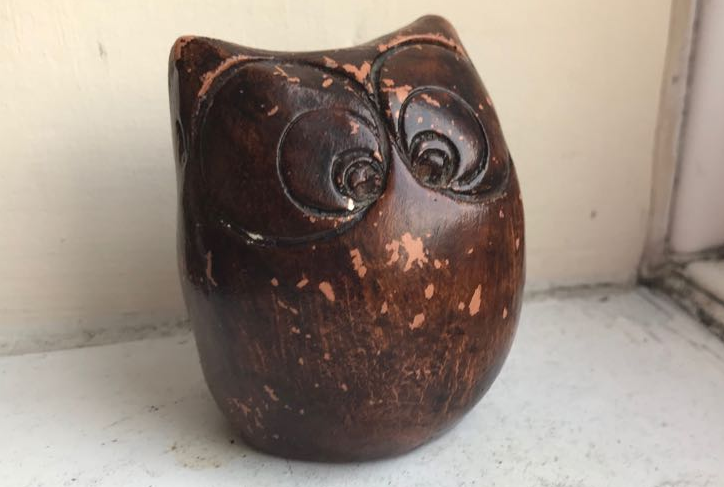
\includegraphics[width=0.7\linewidth]{images/real.png}
 \caption{\label{fig:reference}Photo of the carved owl.}
\end{figure}

I observed these properties from the owl:
\begin{enumerate}
 \item Large carved circles for the eyes.
 \item Variation in the base colour from dark to light brown.
 \item A brushed pattern that shows up more in the light areas
 \item Small and frequent rough scratches.
 \item Larger, less frequent and vein-like scratches.
 \item Lots of chips in the painted coats.
\end{enumerate}

I was unable to find a complete example of a shader similar to what I wish to create, however I was able to find some components scattered across other Shaders. Larry Gritz rusty metal shader\cite{rust} demonstrates one approach towards creating paint flecks. Another Shader by Gritz is the Veined Marble \cite{marble}, which as the name suggests offers an approach to creating vein-like lines throughout a shader. Finally the Rock Material Described by Rasmus Seerup \cite{Rock} shows how we can layer many individual noise components on top of each-other. 

\section{Method Overview} \label{sec:overview}
\subsection{Eyes}
I began by writing a concentric circle shader, which borrows \textit{smoothpulse} and \textit{smoothpulsetrain} from Larry Gritz \cite{larrygritzarman}. These functions produce a repeating pattern of smooth steps up and then down, similar to a sin wave but with flat peaks and dips. A \textit{smoothpulse} is defined by subtracting or multiplying two \textit{smoothsteps} \cite{fundza}. I used the position vector to calculate distance from the origin, this is useful as all points lying on the edge of a circle are the same distance from the centre of that circle.
\begin{algorithm}
\caption{Concentric Circles}\label{alg:concircles}
\begin{algorithmic}[1]
\Procedure{Concentric}{$p, f, g, t$}
\State $r\gets \sqrt[]{p.x^2 + p.y^2}$\Comment{Get the distance from origin}
\State $sum\gets (p.x + p.y)/r$\Comment{Sum the normalized x and y}
\State $period \gets g * sum$
\State \textbf{return} $spte(t, t + period, f, period, r)$
\EndProcedure
\end{algorithmic}
\end{algorithm}
\newline 
Note that \textit{spte} is a wrapper for Larry Gritz function that applies the same fuzz to each side of the \textit{smoothpulse}. The circles in the eye are not concentric, they all share a single point. The circles do not grow linearly; their growth is exponential. To account for these properties I added two new parameters to the algorithm, a warp factor, and an exponent. When warp is zero we get concentric circles, when it is one we get the eye pattern. Exponent determines the growth factor of the circles.
\begin{algorithm}
\caption{Owl eye}\label{alg:owleye}
\begin{algorithmic}[1]
\Procedure{Eye}{$p, f, g, t, w, e$}
\State $recip \gets 1/e$ \Comment{Get the reciprocal of the exponent}
\State $r\gets \sqrt[]{p.x^2 + p.y^2}$\Comment{Get the distance from origin}
\State $sum\gets (p.x + p.y)/r$\Comment{Sum the normalized x and y}
\State $period \gets g * lerp(1, pow(sum,recip), w)$
\State \textbf{return} $spte(t, t + period, f, period, pow(r, recip))$
\EndProcedure
\end{algorithmic}
\end{algorithm}
\newline
 Here we make several modifications, to warp the circles away from being concentric we linearly interpolate between a uniform gap, and $sum^{recip}$ which is what gives us the shared point. Similarly we use $r^{recip}$ as the final parameter to our \textit{smoothpulsetrain} which is what gives us the non-linear growth.
On top of this, noise was added to the return value, and the position p, to give a more natural and imperfect result.

\subsection{Wood}

The wood texture is essentially lots of different types of noise mixed together. I used a large low frequency noise to blend these together, turbulence was also used frequently. To produce the paint chips I defined a \textit{slicednoise} function, which capped the noise at a given value using \textit{smoothstep}. I found that this is very useful for blending my other layers together as most of them are limited to a few spots on the surface. The brush marks were created using turbulence, with noise and y-axis scaling applied to the position. The stretching produced long strands similar to brush marks. I defined another function which was used in the creation of the rough wood cracks and also the veins. This function again  applies scaling in the y-axis to position, but then uses the \textit{slicednoise} function I described earlier; we subtract the return of that function from one, which results in thin lines. These lines are the gaps between the spots of noise created by \textit{slicednoise}. We also get lots of thin, faint lines within the spots themselves.

\subsection{Specular}

To vary the specular I first added a displacement to the whole surface, the value for this was calculated by summing the values of each layer of noise used previously. This gave a texture that directly relates to the distinct markings found on the owl. I then created a subtle noise layer for the specular, which when combined with a roughness layer created by the \textit{slicednoise} function, gives patches of high and low specular, with subtle variations. 

\section{Results} \label{sec:results}
The comparison below shows the result of the eye algorithm described earlier. Followed by a breakdown of the individual layers.

\begin{figure}[htbp]
  \centering
 \subfloat[Concentric circles + noise]{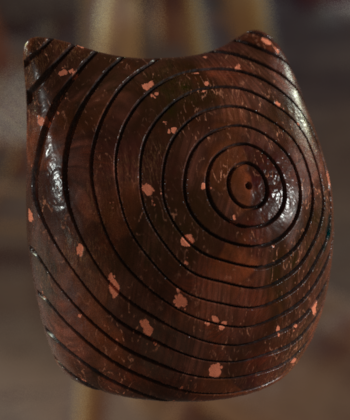
\includegraphics[width=0.49\linewidth]{images/concentric.png}}
 \hfill
 \subfloat[Warped non-linear circles]{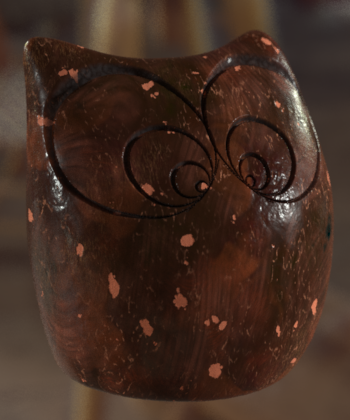
\includegraphics[width=0.49\linewidth]{images/both_eyes.png}}
 \caption{\label{fig:eyecomp}A side by side comparison of the concentric circles function, and the final eye function, with all other parts of the shader enabled.}
\end{figure}

\begin{figure}[htbp]
  \centering
 \subfloat[Base blend noise]{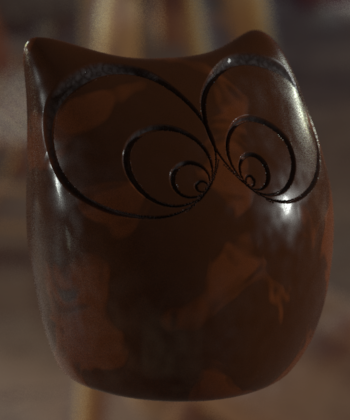
\includegraphics[width=0.32\linewidth]{images/layer_1.png}}
 \hfill
 \subfloat[Roughness and dark spots]{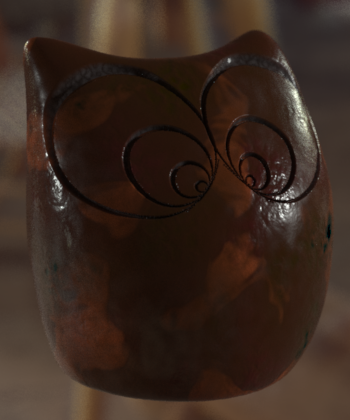
\includegraphics[width=0.32\linewidth]{images/layer_2.png}}
 \hfill
 \subfloat[Brush marks]{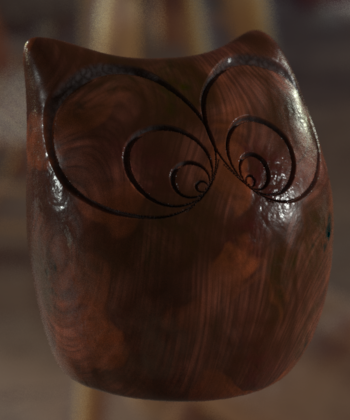
\includegraphics[width=0.32\linewidth]{images/layer_3.png}}
 \vfill
  \subfloat[Light spots and roughness]{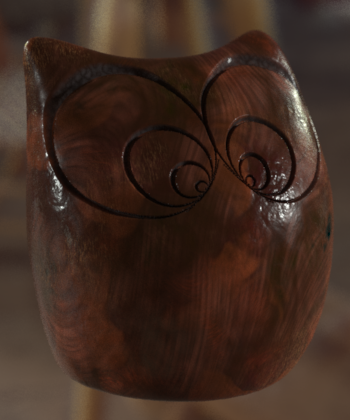
\includegraphics[width=0.32\linewidth]{images/layer_5.png}}
 \hfill
 \subfloat[Vein cracks]{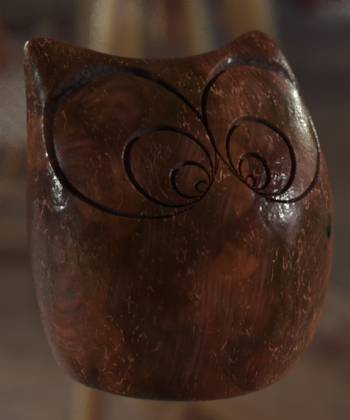
\includegraphics[width=0.32\linewidth]{images/layer_6.png}}
 \hfill
 \subfloat[Paint chips]{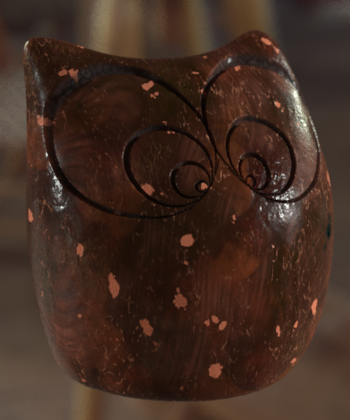
\includegraphics[width=0.32\linewidth]{images/layer_7.png}}
 \caption{\label{fig:layers}Layers enabled one by one.}
\end{figure}

\begin{figure}[ht]
  \centering
 \subfloat[Offset = 0]{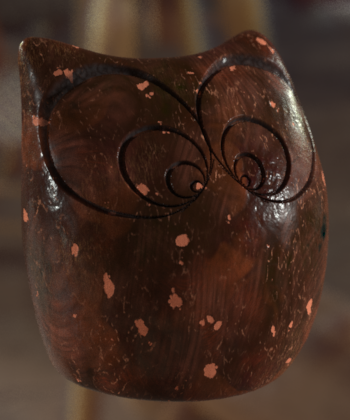
\includegraphics[width=0.425\linewidth]{images/variation_1.png}}
 \hfill
 \subfloat[Offset = 50]{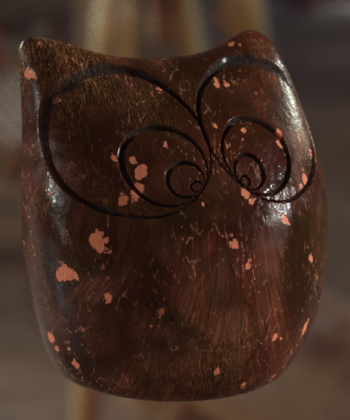
\includegraphics[width=0.425\linewidth]{images/variation_50.png}}
 \hfill
 \subfloat[Offset = 200]{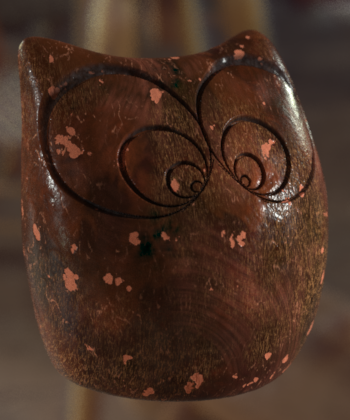
\includegraphics[width=0.425\linewidth]{images/variation_200.png}}
 \hfill
 \subfloat[Offset = 5000]{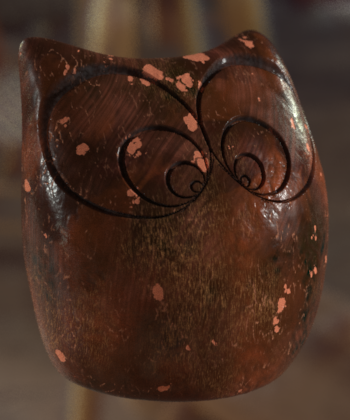
\includegraphics[width=0.425\linewidth]{images/variation_5000.png}}
 \caption{\label{fig:variations}Demonstration of how offsetting the position vector can give a range of outputs due to the procedural nature of the shader.}
\end{figure}

There are several aspects of this shader that I would improve on. The first would be to make the eye mask procedural; dependent on how many circles the user wants. The real object's carved eyes have low spec, high roughness and some extra displacement because they are full of dust. Next I would work on biasing the location of the paint chips so that they always appear around the edge of the eyes. This is again on the real object, and makes sense as hard edges are the most susceptible to wear. Finally I would work on mapping the specular qualities of the shader to the colour of the wood. I observed that on the real object, the specular highlights were weaker and rougher in the dark areas. 

\bibliographystyle{acmsiggraph}
\bibliography{references}


\end{document}
